%---------- Inleiding ---------------------------------------------------------

% TODO: Is dit voorstel gebaseerd op een paper van Research Methods die je
% vorig jaar hebt ingediend? Heb je daarbij eventueel samengewerkt met een
% andere student?
% Zo ja, haal dan de tekst hieronder uit commentaar en pas aan.

%\paragraph{Opmerking}

% Dit voorstel is gebaseerd op het onderzoeksvoorstel dat werd geschreven in het
% kader van het vak Research Methods dat ik (vorig/dit) academiejaar heb
% uitgewerkt (met medesturent VOORNAAM NAAM als mede-auteur).
% 

%TODO nalezen
\section{Inleiding}%
\label{sec:inleiding}

De dag van vandaag focust de zorg- en welzijnssector vooral op persoonsgerichte zorgverlening. Dit impliceert dat de zorgverleners hun communicatiestijl aanpassen aan de zorgvragers. In de context van zorgverlening bij ouderen wordt de communicatiestijl echter vaak als te betuttelend ervaren. Men noemt dit fenomeen secondary babytalk of elderspeak. Om dit tegen te gaan, wil de opleiding verpleegkunde aan HOGENT gebruik maken van een applicatie die zou helpen om via speech-to-text de secondary babytalk op te sporen. Aan de hand daarvan zouden ze dan feedback kunnen geven aan de studenten tijdens praktijksessies in het Zorglab.

Het Zorglab is een lokaal dat voornamelijk gebruikt wordt tijdens de praktijklessen in de opleiding verpleegkunde. Het lokaal bestaat uit 2 ruimtes waarin camera's hangen. De studenten kunnen hier microfoons dragen zodat medestudenten in een derde ruimte kunnen volgen wat er gebeurt en ondertussen feedback krijgen van de lector. Hier zou dus gebruik gemaakt worden van de applicatie om snel de voorvallen van elderspeak op te sommen zodat de studenten ook feedback kunnen krijgen op wat ze zelf gedaan hebben en niet enkel op wat studenten in een andere groep doen.

In voorgaande jaren werd in de bachelorproeven van \textcite{Govaerts2022}, \textcite{Gussem2022} en \textcite{Daems2023} reeds succesvol een applicatie ontwikkeld die signalen van elderspeak kan herkennen aan de hand van kenmerken zoals toonhoogte en stemvolume. In deze applicatie kan men een audiofragment uploaden en dit aan de hand van een aantal parameters laten analyseren. In de jaren die daarop volgden werd er in de bachelorproeven van \textcite{Branden2024}, \textcite{Coetsiers2024} en \textcite{Schryver2024} onderzoek gedaan naar het integreren van een model dat spraak kan omzetten naar tekst, maar hier werd aangetoond dat de accuraatheid van bestaande modellen onvoldoende blijkt te zijn om een kwaliteitsvolle transcriptie uit te voeren van gesproken Nederlands.

Deze bachelorproef zal focussen op het onderscheiden van verschillende stemmen. \hl{De hoofdvraag die hierbij gesteld wordt, is: kan ervoor gezorgd worden dat de applicatie onderscheid maakt tussen de stem van de zorgverlener en die van de zorgvrager? Dit kan opgesplitst worden in verschillende deelvragen:}
\begin{itemize}
	\item \hl{Wat zijn reeds bestaande modellen en python libraries die stemmen kunnen herkennen en onderscheiden?}
	\item \hl{Wat zijn de beste parameters om een model te trainen op het onderscheiden en afzonderen van stemmen?}
	\item \hl{Is het mogelijk om het getrainde model in de applicatie te integreren?}
\end{itemize}
Dit heeft als einddoel om de reeds bestaande applicatie uit te breiden met de mogelijkheid om te focussen op de stem van de zorgverlener voor het opsporen van signalen van secondary baby talk.

%---------- Stand van zaken ---------------------------------------------------

%TODO verdere subsecties maken en literatuur opzoeken
\section{Literatuurstudie}%
\label{sec:literatuurstudie}

\subsection{Voorgaand onderzoek in verband met de applicatie}%

In voorgaande bachelorproeven werd reeds een applicatie ontwikkeld met als doel deze te gebruiken in de opleiding verpleegkunde. Volgens \textcite{Govaerts2022} is het detecteren van elderspeak mogelijk met behulp van PRAAT en Natural Language Processing (NLP). PRAAT is een computerprogramma voor het analyseren, synthetiseren en manipuleren van spraak en werd ontwikkeld sinds 1992 door Paul Boersma en David Weenink \autocite{Govaerts2022}.

Datzelfde jaar werd door \textcite{Gussem2022} geconcludeerd dat elderspeak gedetecteerd kan worden met AI. De software die hiervoor beschikbaar is, is echter gelimiteerd en niet altijd accuraat en kan de stem van de zorgvrager niet wegfilteren voor de analyse \autocite{Gussem2022}.

Later onderzocht \textcite{Daems2023} hoe de detectie van elderspeak verbeterd kan worden door het toepassen van een ruisfilter en een stiltefilter. De conclusie omtrent de ruisfilter was dat deze zeker helpt, maar niet alle ruis uit het signaal kan verwijderen \autocite{Daems2023}. Om dit te verbeteren opperde \textcite{Daems2023} dat het gebruik van meerdere microfoons zou kunnen helpen.
Wanneer het gaat over de stiltefilter, besloot \textcite{Daems2023} dat deze succesvol de stiltes kan detecteren en analyseren, wat het mogelijk maakt om stiltes te verwijderen en andere parameters te verbeteren. \textcite{Daems2023} concludeerde echter ook dat factoren zoals geluidskwaliteit, gesproken dialect, linguïstische verschillen en het doel voor de spraakherkenning de kwaliteit ervan ook sterk beïnvloeden.

\textcite{Branden2024} zocht naar verdere mogelijkheden om de accuraatheid van elderspeak detectie te verhogen. Uit dit onderzoek kon geconcludeerd worden dat het gebruik van een POS-tagger ervoor zorgde dat de accuraatheid significant verhoogd werd, namelijk van 92.71\% naar 99.48\% \autocite{Branden2024}. POS-tagging is een NLP techniek waarbij woordsoorten worden toegekend aan woorden of tokens en hierbij ook rekening houdt met de context \autocite{Branden2024}.

Het onderzoek van \textcite{Schryver2024} had als doel om spraak naar tekst om te zetten. Hieruit moest echter de conclusie getrokken worden dat het accuraat omzetten van gesproken naar geschreven tekst nog niet mogelijk is \autocite{Schryver2024}. \textcite{Schryver2024} onderzocht ook of er mogelijkheden zijn om de performantie van de applicatie te kunnen verbeteren aangezien deze momenteel eerder traag is, maar de conclusie was dat dit niet het geval lijkt te zijn.

\subsection{Onderzoek naar het onderscheiden van stemmen}

Er zijn al verschillende onderzoeken gebeurd om stemmen te onderscheiden in audio fragmenten. \textcite{Zeghidour2021} hebben een model ontworpen dat gebruik maakt van 2 convolutionele subnetwerken om zo succesvol de verschillende signalen van elkaar te onderscheiden. Het eerste subnetwerk is een 'speaker stack', die de input in kaart brengt aan de hand van een set vectoren. Het tweede subnetwerk is een 'separation stack', die gebruik maakt van de input en de vector representaties. De combinatie van deze 2 subnetwerken zorgt ervoor dat het model een representatie van elke bron maakt en op basis hiervan een schatting maakt van de gescheiden signalen. \autocite{Zeghidour2021}

Een ander onderzoek werd gedaan door \textcite{Nachmani2020}, waar ze geprobeerd hebben om het 'cocktail party probleem' op te lossen. Het 'cocktailparty probleem' is een probleem waarbij het voorkomen van veel occluderende instanties het moeilijk maakt om te segmenteren. \textcite{Nachmani2020} zien hier echter dat spraaksignalen ook stille delen bevatten en het segmenteren dus niet kan gebeuren op basis van continuïteit alleen. Hierdoor hebben \textcite{Nachmani2020} ook een op identificatie gebaseerde component voor het verlies aan constantheid toegevoegd. Dit werd bereikt door het toevoegen van een nieuw recurrent blok, dat bestaat uit een combinatie van twee bidirectionele RNN's en een skip connectie, het gebruik van verschillende verlies functies en een spraakconstantieterm \autocite{Nachmani2020}.

\textcite{Nandal2019} zocht naar een manier om stemmen te onderscheiden aan de hand van deep learning technieken. Ze deed dit door gebruik te maken van de SHOGUN machine learning toolbox en gebruikte het JADE (Joint Approximate Diagonalization of Eigenmatrices) algoritme voor de onafhankelijke componenten analyse \autocite{Nandal2019}. SHOGUN is een open source machine learning toolbox die kan gebruikt worden voor zowel supervised als unsupervised learning en bevat een uitgebreide reeks krachtige en uniforme machine learning methoden \Autocite{Nandal2019}. Het probleem waar \textcite{Nandal2019} op botste, was het feit dat de maximale lengte van de fragmenten die ze kon gebruiken slechts 3 seconden was.

In een onderzoek van \textcite{Li2021} werd onderzocht hoe de onderscheiding kon gebeuren op langere opnames. Hiervoor maakten ze gebruik van een reeds bestaande techniek om de opname te segmenteren in kortere blokken waarop het onderscheiden dan op de verschillende blokken in parallel gebeurt\autocite{Li2021}. Het probleem bij deze methode is dat een deel van de afhankelijkheden tussen de verschillende blokken verloren gaat, waardoor \textcite{Li2021} besloten om gebruik te maken van dual-path RNN (DPRNN). Dit leverde voornamelijk significante verbeteringen op voor blokken met kleinere groottes, waardoor \textcite{Li2021} concludeerden dat het gebruik van een DPRNN voornamelijk geschikt is voor systemen die een kleine latency vereisen.

%---------- Methodologie ------------------------------------------------------
\section{Methodologie}%
\label{sec:methodologie}

Het onderzoek zal starten met een literatuurstudie. Het grootste deel hiervan zal bestaan uit het opzoeken van reeds bestaande modellen om stemmen te herkennen in audiofragmenten en het bekijken of deze al dan niet bruikbaar zijn in dit onderzoek. Er zal ook gezocht worden naar eventueel bestaande python libraries die gebruikt kunnen worden.

De tweede fase van het onderzoek zal bestaan uit het trainen van modellen en het zoeken naar de ideale parameters. Voor het trainen zullen we starten met audiofragmenten waar weinig tot geen ruis aanwezig is en waar het onderscheid tussen de 2 stemmen duidelijk is, zoals bijvoorbeeld door audio te gebruiken met de stem van een man en een vrouw. In een volgende stap zullen audiofragmenten gebruikt worden waar de stemmen minder duidelijk van elkaar te onderscheiden zijn, zoals bijvoorbeeld 2 mannen of 2 vrouwen. Hierna zullen fragmenten gebruikt worden waar opzettelijk ruis aan toegevoegd is, om uiteindelijk te eindigen met de audiofragmenten die opgenomen zijn in het Zorglab voor voorgaande bachelorproeven. Om te weten of alle stappen in deze fase geslaagd zijn, zullen de stemmen in de audiofragmenten op voorhand gelabeld worden. Aan de hand van deze labels kan dan achteraf gecontroleerd worden of de scheiding van de stemmen correct gebeurd is. Het beslissen welk model uiteindelijk gebruikt zal worden, zal gebeuren aan de hand van technieken om de accuraatheid van een model te bekijken, zoals MSE (Mean Squared Error). Het model dat het beste scoort, zal verder gebruikt worden.

Tot slot zal er een manier gezocht worden om het getrainde model te integreren in de reeds bestaande applicatie, zodat deze het model kan gebruiken om enkel op de stem van de zorgverlener (in opleiding) te focussen.

Om een beter zicht te geven op verloop van het onderzoek voor deze bachelorproef, bevat Figuur 1 een flowchart die een overzicht biedt voor het verloop van de hierboven beschreven stappen. In Figuur 2 wordt een tijdsinschatting gemaakt voor elke fase.

\begin{figure}
	\centering
	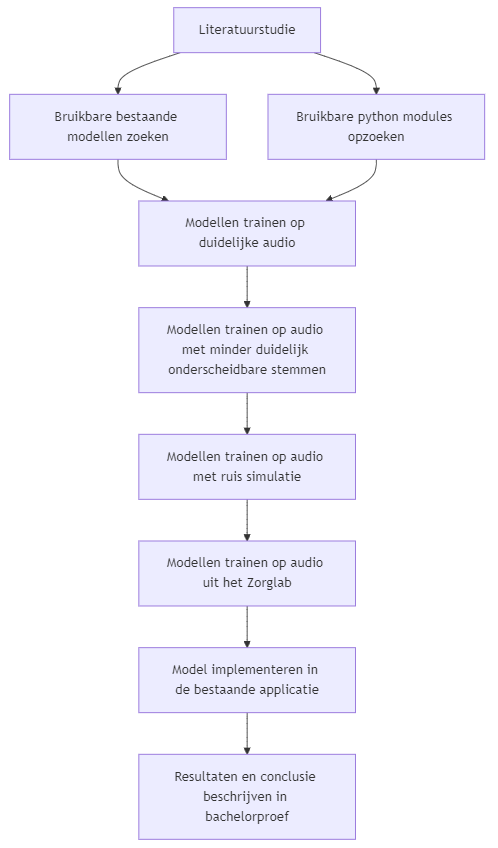
\includegraphics[width=\columnwidth]{img/flowchart.png}
	\caption{Flow chart}
\end{figure}

\begin{figure*}
	\centering
	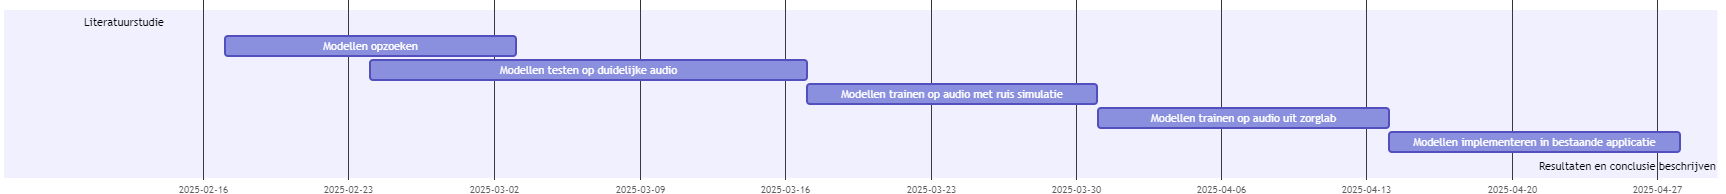
\includegraphics[width=\textwidth]{img/gantt.png}
	\caption{Gantt chart}
\end{figure*}

%---------- Verwachte resultaten ----------------------------------------------
\section{Verwacht resultaat, conclusie}%
\label{sec:verwachte_resultaten}

Als eindresultaat van de literatuurstudie worden een of meerdere modellen en python libraries verwacht waarvoor getest kan worden of ze bruikbaar zijn voor deze bachelorproef.

Het verwachte resultaat van het trainen van modellen is bij elke tussenstap een model dat succesvol stemmen kan onderscheiden, een audiofragment teruggeeft met enkel de gewenste stem en verder getraind en verfijnd kan worden in de volgende tussenstappen. Het verwachte resultaat van de laatste stap in deze fase is een model dat succesvol stemmen kan onderscheiden in de audio die opgenomen wordt in het Zorglab en geïmplementeerd kan worden in de reeds bestaande applicatie.

Het verwachte eindresultaat van deze bachelorproef is een succesvolle integratie van het getrainde model in de reeds bestaande applicatie, waardoor deze uiteindelijk de optie biedt om enkel te focussen op de stem van de zorgverlener.
